To construct $\mathtt{h}$, we evaluate the integral of the logarithm using quadrature.
For an integral on the real line, Gaussian quadrature approximates it by transforming it to the unit ball,
\[
\int_{a}^{b} y(x) \,\dee x \mapsto \int_{-1}^{1} \eta(\xi) \,\dee\xi,
\]
where $\eta(\xi) \equiv y\big( x(\xi) \big) \partial_{\xi}x$, a change of variables such that $x(-1) = a$ and $x(1) = b$.
\textsc{Gauss}--\textsc{Legendre} quadrature of order $K$ has us approximating this integral by
\[
\sum_{k = 1}^{K} w_k \eta(\xi_k), \quad w_k = \frac{2}{\big( 1 - {\xi_k}^2 \big) {\big( {\legendre_K^{\prime}(\xi_k)} \big)}^2},
\]
where $\legendre_K$ is the $K$\textsuperscript{th} \textsc{Legendre} polynomial, $\xi_k$ is its $k$\textsuperscript{th} zero, and $w_k$ is the corresponding weight.
The \textsc{Legendre} polynomials are given by the recursion formula\footnote{\cite{abramowitz1965handbook} \textsc{Abramowitz} \& \textsc{Stegun}, 22.7.10, p.782}
\[
(n + 1) \legendre_{n+1}(\xi) = (2n + 1) \xi \legendre_{n}(\xi) - n\legendre_{n-1}(\xi),
\]
where we have defined $\legendre_0(\xi) = 1$, $\legendre_1(\xi) = \xi$.
From the recurrence relation we find the 2\textsuperscript{nd} order \textsc{Legendre} polynomial, its zeros, and its weights:
\[
\legendre_2(\xi) = \frac{3x^2 - 1}{2}, \quad \xi_k = {(-1)}^k \frac{\sqrt{3}}{3}, \quad w_k = 1
\]
We find below that we have no use for the 3\textsuperscript{rd} polynomial, but we may use the 4\textsuperscript{th}, for which we have
\[
\legendre_4(\xi) = \frac{105\xi^4 - 90\xi^2 + 9}{24}, \quad \xi_k = \pm\sqrt{\frac{3 \pm 2\sqrt{\sfrac{6}{5}}}{7}}.
\]
The zeros $\xi_k$ are readily found by solving the biquadratic equation, the the signs may be chosen independently, yielding four roots.
As for the wieghts, they are found after some algebraic manipulation, and turn out to be
\[
w_k = \frac{18 \pm \sqrt{30}}{36}.
\]
Instead of ginning up some elaborate mathematical expression to relate the roots to their respective weights, an illustration is provided in figure \ref{fig:fourth_legendre} below.
\begin{Figure}
  \centering
  \scalebox{1}{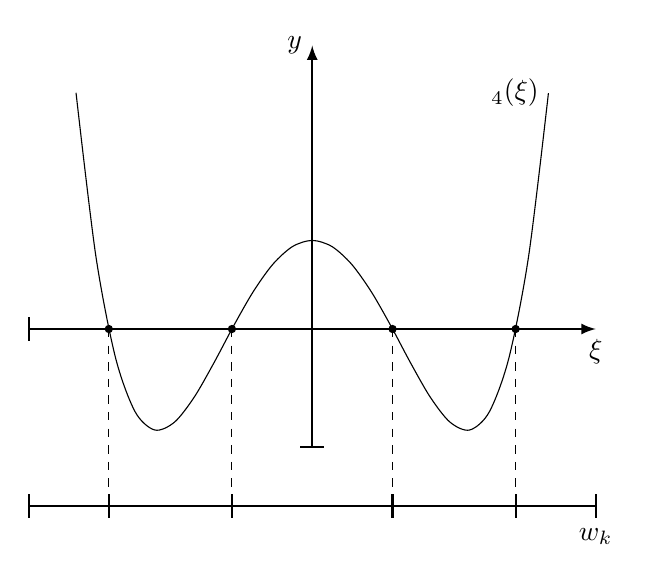
\begin{tikzpicture}
  \begin{scope}[scale = 3]
    \def\xmax{1.2}
    \def\ymin{-.5}
    \draw[-latex, thick] (-\xmax, 0)--(\xmax, 0) node[below]{$\xi$};
    \draw[thick] (-\xmax, .05)--(-\xmax, -.05);
    \draw[-latex, thick] (0, -.5)--(0, \xmax) node[left]{$y$};
    \draw[thick] (-.05, \ymin)--(.05, \ymin);
    \draw[domain = -1:1] plot[smooth] (\x, {4.375*(\x)^4 - 3.75*(\x)^2 + .375}) node[left]{$\legendre_4(\xi)$};
    \def\weightline{-.75}
    \draw[thick] (-\xmax, \weightline)--(\xmax, \weightline) node[below = 1ex]{$w_k$};
    \draw[thick] (-\xmax, {\weightline + .05})--(-\xmax, {\weightline - .05});
    \draw[thick] (\xmax, {\weightline + .05})--(\xmax, {\weightline - .05});
    \foreach \k in {1,2} {
      \foreach \x in {0.861136, 0.339981} {
        \def\xcoord{{(-1)^(\k) * \x}}
        \draw[fill = black] (\xcoord, 0) circle (.015);
        \draw[dashed] (\xcoord, 0) -- (\xcoord, \weightline);
        \ifthenelse{\equal{\x}{0.861136}}{%
          \def\fraction{$\frac{18-\sqrt{30}}{36}$}
        }{%
          \def\fraction{$\frac{18+\sqrt{30}}{36}$}
        }
        \draw[thick] (\xcoord, {\weightline + 0.05})--(\xcoord, {\weightline - 0.05}) node[below]{\fraction};
      }
    }
  \end{scope}
\end{tikzpicture}
}
  \captionsetup{type = figure}
  \caption{The fourth \textsc{Legendre} polynomial plotted, with the weights associated with its four roots indicated.}
  \label{fig:fourth_legendre}
\end{Figure}

To calculate the target integral by quadrature, we may parametrize the variable of integration by writing that the line segment $S_n$ is given by
\[
\ezh(\xi) = \left( \frac{\xvec_n - \xvec_{n-1}}{2} \right)\xi + \left( \frac{\xvec_{n} + \xvec_{n-1}}{2} \right),
\]
where $\xi \in [-1,1]$.
We recognize the right-most term above as $\zhett_n$, and for brevity, we write that $\xvec_{n} - \xvec_{n-1} = \dxtt$, which is implemented as the method \texttt{IntegralEquation.\textDelta{x}}.
Now $\ln{\absl{\ezh(\xi)}}$ clearly is a function from the real numbers into the real numbers, so we may use the fact that for any real valued function over the complex plane,
\[
\int_{C} f(\ezh) \,\dee S = \int_{a}^{b} f\big( \ezh(\xi) \big) \absl{\ezh^{\prime}(\xi)} \,\dee\xi.
\]
We calculate that $\absl{\ezh^{\prime}(\xi)} = \sfrac{1}{2}\absl{\dxtt}$, which is implemented as the class variable $\mathtt{dS}$ in the \texttt{Quadrature} class of \texttt{quadrature.py}.
It should now be clear that we may not use an odd order quadrature scheme, as the diagonal of $\mathtt{h}$ will entail evaluating the logarithm at zero, since $\xi_k = 0$ will always be a root of an odd order \textsc{Legendre} polynomial.

We again utilize the fact that $\Re{\big( \log{\ezh} \big)} = \ln{\absl{\ezh}}$, so that
\[
\int_{S_n} \ln{r} \,\dee S = \frac{\absl{\dxtt}}{2} \Re\int_{-1}^{1} \log{\big( \ezh(\xi) -\bzhe_m \big)} \,\dee\xi,
\]
the latter of which we may employ quadrature on.
